\chapter{Implementarea Sistemelor de Fișiere}

\section{Simularea disk-ului}

\subsection{Inițierea disk-ului}

Pentru a putea simula disk-ul, vom crea un folder în cadrul sistemului de fișiere oferit de sistemul de operare pe care vor fi rulate mai apoi cele 3 sisteme de fișiere. Acest folder conține 2 fișiere simple, fără extensie: un fișier 'Metadata', care oferă informațiile necesare inițierii simulării (cum ar fi numarul de sectoare ale hard disk-ului si dimensiunea in bytes a fiecarui sector), odată ce aceasta a fost deja creată într-o dată anterioară, și un alt fișier 'Data', care reprezintă disk-ul simulat. Acest fișier este în esență doar un șir de caractere, care vor reprezenta byții din cadrul disk-ului nostru.

Pentru crearea celor două fișiere, precum și pentru scrierea și citirea acestora, a fost necesară utilizarea API-ului oferit de sistemul de operare în cadrul căruia este dezvoltată această lucrare de licență, și anume Windows 10. Acesta ne pune la dispoziție o serie de metode pentru manipularea fișierelor, prin intermediul bibliotecii "windows.h".

\bigskip

\begin{figure}[h]
    \centering
    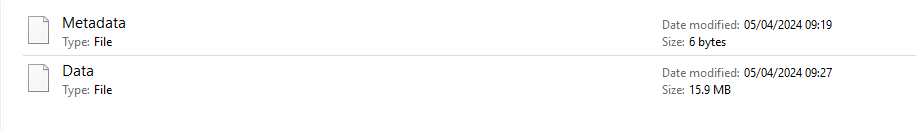
\includegraphics[width=1.0\linewidth]{images/2.1.png}
    \caption{Disk-ul simulat}
    \label{fig:enter-label}
\end{figure}

În momentul în care este creat disk-ul, acesta nu conține nicio informație, toți byții fiind setați la 0. Pentru a realiza acest lucru în cadrul simulării, după crearea celor două fișiere, vom umple fișierul 'Data' cu caracterul null (adică valoare 0), în conformitate cu dimensiunea disk-ului, și anume (numărul de sectoare) * (dimensiunea unui sector). Aceste valori vor fi oferite ca și input de către utilizator la crearea disk-ului, împreună cu locația unde se dorește salvarea acestuia.


\begin{figure}[h]
    \centering
    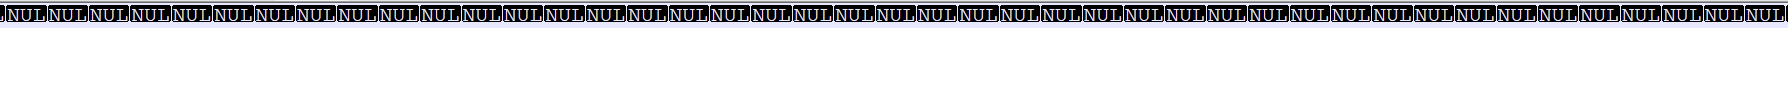
\includegraphics[width=1.0\linewidth]{images/2.2.png}
    \caption{Vizualizare a disk-ului după creare}
    \label{fig:enter-label}
\end{figure}


\subsection{Scrierea si citirea sectoarelor}

Pe lângă crearea și inițierea disk-ului, biblioteca pe care o creăm pune la dispoziție, în mod evident și o serie de funcții care ajută la scrierea și citirea datelor aflate pe disk. Scrierea și citirea byților a fost realizată într-un mod care să simuleze felul în care datele sunt extrase și modificate de pe un disk real, bineînțeles cu limitările pe care ni le impune faptul că în realitate lucrăm cu un fișier aflat în cadrul sistemului de operare Windows 10, și nu cu o componentă hardware adevărată. Astfel, fiecare operațiune de scriere sau citire afectează întregul conținut al unui sector, sau a mai multor sectoare consecutive.

Să luăm ca și exemplu, un disk care are dimensiunea sectoarelor de 512 bytes. În cazul în care dorim să citim byții aflați între adresele 800 și 1200, noi vom citi de fapt toți byții de la adresa 512 până la 1535, adică sectoarele 1 și 2 în totalitate (indexarea sectoarelor făcându-se de la 0), același lucru întâmplându-se și în cazul operației de scriere.

\bigskip

\lstset{style=code-snyppet-style}
\begin{lstlisting}
static int readSector(DiskInfo *diskInfo, uint32_t sector, char *buffer)
{
    char *fullFilePath = buildFilePath(diskInfo->diskDirectory);

    HANDLE fileHandle = CreateFile(fullFilePath,OFN_READONLY,0,nullptr,
                          OPEN_EXISTING, FILE_ATTRIBUTE_NORMAL,nullptr);

    if(fileHandle == INVALID_HANDLE_VALUE)
    {
        CloseHandle(fileHandle);
        delete[] fullFilePath;
        return SECTOR_READ_FAILED;
    }

    OVERLAPPED overlapped;
    memset(&overlapped, 0, sizeof(OVERLAPPED));
    overlapped.Offset = diskInfo->diskParameters.sectorSizeBytes * sector;
    overlapped.hEvent = nullptr;

    DWORD dwBytesRead = 0;
    bool readFileResult = ReadFile(fileHandle, buffer, 
        diskInfo->diskParameters.sectorSizeBytes, &dwBytesRead, &overlapped
        );

    if(!readFileResult || dwBytesRead < diskInfo->diskParameters.sectorSizeBytes)
    {
        CloseHandle(fileHandle);
        delete[] fullFilePath;
        return SECTOR_READ_FAILED;
    }

    CloseHandle(fileHandle);
    delete[] fullFilePath;

    return SECTOR_READ_SUCCESS;
}
\end{lstlisting}

\subsection{Probleme intâmpinate}

Ideea din spatele acestei simulări a fost încă de la început aceea de a putea fi folosită, într-un stil similar, de toate cele 3 sisteme de fișiere care vor fi implementate folosindu-se de funcționalitățile oferite de aceasta. Astfel, în momentul finalizării librăriei, aceasta a trebuit să pună la dispoziție o interfață care urma să fie folosită în cadrul celor 3 proiecte, fără a mai fi schimbată ulterior, pentru a nu trebui să facem modificări în cadrul sistemelor de fișiere, datorită faptului că simularea disk-ului a suferit schimbări (adică s-a dorit ca toate modificările ulterioare să fie backwards compatible). Mai jos se poate vedea API-ul pus la dispoziție de către  librărie, acesta nesuferind nicio modificare ulterioară de-a lungul dezvoltării acestei lucrări de licență.

\bigskip

\lstset{style=code-snyppet-style}
\begin{lstlisting}
DiskInfo* initializeDisk(const char* diskDirectory, uint32_t sectorsNumber, uint16_t sectorSize);

int fillDiskInitialMemory(DiskInfo *diskInfo, uint32_t batchSize);

DiskInfo* getDisk(const char* diskDirectory);

int getDiskStatus(DiskInfo *diskInfo);

int readDiskSectors(DiskInfo *diskInfo, uint32_t numOfSectorsToRead, uint32_t sector, char* buffer, uint32_t &numOfSectorsRead);

int writeDiskSectors(DiskInfo *diskInfo, uint32_t numOfSectorsToWrite, uint32_t sector, char buffer[], uint32_t &numOfSectorsWritten);
\end{lstlisting}

\bigskip

Deși această interfață a fost gândită astfel încât să nu necesite modificări ulterioare, asta nu înseamnă că implementarea sa nu a trecut prin anumite schimbări de-a lungul timpului. Pe lângă mici bug-uri care au fost reparate, cum ar fi ștergerea unui pointer null, sau dealocarea la momentul inoportun a unui buffer folosit la scrierea/citirea datelor, a fost necesară și o regândire totală a modului în care sectoarele sunt definite în cadrul simulării.

Așa cum am văzut mai sus, în momentul actual disk-ul în sine, este simulat cu ajutorul unui singur fișier 'Data', care conține toți byții din cadrul său, sectoarele nefiind separate în mod 'fizic' în interiorul acestui fișier, distincția dintre ele făcându-se doar la nivel logic. Acesta nu a fost însă cazul încă de la început, implementarea inițială presupunând existența unui fișier separat pentru fiecare sector în parte.

\bigskip

\begin{figure}[h]
    \centering
    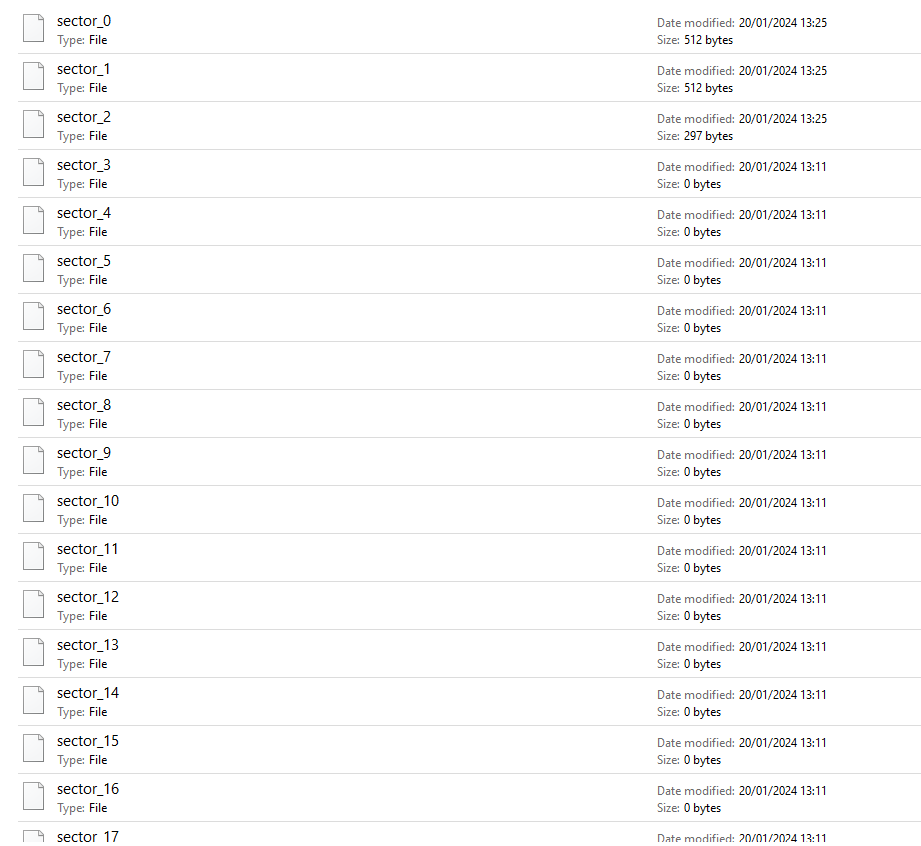
\includegraphics[width=1.0\linewidth]{images/2.3.png}
    \caption{Implementarea inițială a disk-ului}
    \label{fig:enter-label}
\end{figure}

\bigskip

De ce am făcut această schimbare drastică? Ei bine, în timpul dezvoltării primului dintre cele 3 sisteme de fișiere, și anume FAT32, am observat probleme legate de timpul necesar creării disk-ului. Inițial am ignorat acest lucru, întrucât în cadrul dezvoltării erau suficiente disk-uri de dimensiuni reduse (512 KiB) pentru testele pe care le făceam, astfel și timpul inițierii fiind unul redus, însă odată cu evoluția implementării, teste pe fișiere de dimensiuni mai ample au devenit necesare, astfel și dimensiunea disk-ului trebuind să crească în mod corespunzător. În acest moment, problemele legate de performanța instanțierii disk-ului au devenit tot mai vizibile, devenind chiar un impediment major în procesul de testare. Spre exemplu, crearea unui disk de 1 GiB dura inițial aproximativ 30 de minute, spre deosebire de câteva secunde, cât durează cu implementarea actuală, care folosește un fișier comun, și nu câte unul pentru fiecare sector.

Problemele de performanță, însă, nu erau cauzate doar de existența unui număr ridicat de fișiere, ci și a modului în care se realiza popularea inițială a datelor din cadrul disk-ului, cu caracterul null (valoarea 0).

\bigskip

\lstset{style=code-snyppet-style}
\begin{lstlisting}
int fillDiskInitialMemory(DiskInfo *diskInfo, uint32_t batchSize);
\end{lstlisting}

\bigskip

Astfel, au existat 3 moduri de 'umplere' a disk-ului, până să se ajungă la varianta finală, care este bineînțeles și cea mai eficientă.

\begin{itemize}
  \item \textbf{Popularea fiecărui fișier ce constituia un sector}, aceasta fiind varianta folosită în cadrul implementării inițiale, care folosea câte un fișier separat pentru reprezentarea fiecărui sector, și astfel, scrierea acestora făcându-se în mod independent.
  
  \item \textbf{Popularea independentă a fiecărui sector logic}, aici vorbim deja de cea de-a doua implementare a disk-ului, care folosește un singur fișier, și unde sectoarele sunt separate doar la nivel logic. Cu toate acestea, popularea fiecărui sector se realiza separat, acest lucru presupunând un număr ridicat de operațiuni de deschidere, scriere și apoi închidere asupra fișierului 'Data', ceea ce ducea la o performanță scăzută.
  
  \item \textbf{Popularea sectoarelor în batch-uri}, această variantă finală presupune exploatarea faptului că sectoarele nu sunt separate în mod fizic, ci sunt poziționate consecutiv în interiorul fișierului 'Data'. Astfel, pentru a reduce numărul operațiunilor asupra acestui fișier, popularea lor se realizează în batch-uri de mai multe sectoare.
  
\end{itemize}



















\newpage

\section{FAT32}

\subsection{Privire de ansamblu asupra FAT32}

FAT32 este un sistem de fișiere relativ simplu, care presupune utilizarea unei tabele de indici (File Allocation Table) pentru înlănțuirea unor blocuri de date numite clustere. Din punct de vedere structural, FAT32 se împarte în 4 regiuni:

\begin{itemize}
  \item \textbf{Reserved Area}, această zonă conține date necesare pentru pornirea și funcționarea sistemelor din cadrul calculatorului. În prima parte a acestei regiuni se află 'Boot Record', care conține codul ce trebuie executat inițial pentru pornirea sistemului, totodată aici aflându-se o serie de structuri de date necesare sistemului nostru de fișiere, și anume BIOS Parameter Block (BPB), Extended Boot Record și FSInfo.
  
 \item \textbf{FAT 1}, regiune ce reprezintă tabela de indici menționată mai sus. Aceasta conține o serie de valori de 32 de biți (dintre care doar ultimii 28 sunt luați în considerare, primii 4 fiind ignorați), fiecare astfel de valoare reprezentând numărul următorului cluster în cadrul înlănțuirii actuale (a directorului curent). Spre exemplu, dacă la indexul 16 (adică byte-ul 64) se află valoarea 783, înseamnă că datele aflate în continuarea celor din cluster-ul 16 se află în cluster-ul 783.
 
 \item \textbf{FAT 2}, este o copie a FAT 1, servind în special ca și un backup, în cazul posibilelor erori ce pot apărea în tabela principală.
 
 \item \textbf{Data Area}, această regiune conține datele propriu-zise, înglobând folderele și fișierele stocate. Prima parte a acestei zone este numită 'Root directory', și se comportă ca un director obișnuit, acesta putând conține atât sub-foldere cât și fișiere. Aspectul distinctiv al acestuia însă, este faptul că este singurul director ce nu are un părinte, el reprezentând rădăcina arborelui de directoare stocate în cadrul sistemului de fișiere.  
\end{itemize}


\begin{figure}[h]
    \centering
    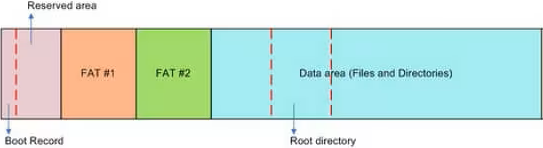
\includegraphics[width=1.0\linewidth]{images/2.4.png}
    \caption{Structura FAT32}
    \label{fig:enter-label}
\end{figure}

\bigskip


\subsection{Modul de implementare}

Fiind în esență doar o simulare (la fel ca toate cele 3 sisteme de fișiere din cadrul acestei lucrări), implementarea FAT32 a trebuit adaptată astfel încât să funcționeze fără a avea acces la hardware, ci doar la disk-ul nostru simulat, și fără a face parte dintr-un sistem de operare. Singura interacțiune de acest fel este una indirectă, prin intermediul simulării disk-ului, atunci când se realizează operațiuni asupra datelor stocate de acesta.

Din aceste considerente, simularea de FAT32 rulează sub forma unui program, cu care utilizatorul poate interacționa prin intermediul terminalului. Așa cum am precizat și mai sus, simularea noastră nu are legătură în mod direct cu sistemul de operare, ca în cazul unui sistem de fișiere adevărat. Aceasta duce la imposibilitatea ca structurile de date de care avem nevoie în cadrul FAT32 să se afle în mod permanent în memorie (RAM), și totodată la lipsa unor procese special dedicate care să ruleze în momentul în care se dorește realizarea unei operațiuni asupra disk-ului (cum ar fi scrierea sau citirea datelor). De aceea, am considerat ca rularea programului de simulare este singura soluție viabilă in cazul nostru, pentru a putea interacționa cu sistemul de fișiere.


\subsubsection{Inițializarea FAT32}

În momentul în care programul este rulat, acesta parcurge mai multe etape in vederea pregatirii disk-ului, cat si a sistemului de fișiere propriu-zis:

\begin{enumerate}
  \item \textbf{Verificarea existenței disk-ului}, aici se verifică dacă disk-ul a fost deja inițializat la locația dată ca și parametru.

  \item \textbf{Inițializarea/Citirea disk-ului}, această etapă depinde de rezultatul pasului anterior. Dacă simularea disk-ului nu a fost găsită la locația precizată, acesta este instanțiat: se creează fișierele 'Metadata' și 'Data', acesta din urmă fiind populat cu null (valoarea 0), în conformitate cu dimensiunea dorită. Dacă disk-ul a fost deja inițiat, atunci se citesc datele referitoare la acesta și se stochează într-o structură de date, DiskInfo, care ne va fi de folos pe parcurs.

  \item \textbf{Verificarea inițializării sistemului de fișiere}, acest pas realizează citirea primului sector de pe disk, adică a sectorului de bootare. Dacă la finalul acestui sector se află semnătura specifică sistemului de fișiere FAT32, și anume 0xAA55, înseamnă că sistemul a fost deja inițiat, sau nu, in caz contrar.

  \item \textbf{Inițializarea sistemului de fișiere}, etapă ce are loc doar în cazul în care verificarea de mai devreme returnează fals. În cadrul acestui pas sunt create datele din cadrul BIOS Parameter Block și a Extended Boot Record, care vor fi stocate împreună în cadrul unei structuri numite BootSector, pentru ca mai apoi să fie salvate în sectorul de bootare (sectorul 0), bineînțeles împreună cu semnătura reprezentativă FAT32 despre care am vorbit mai sus. Tot aici este creată o altă structură de date, FSInfo, aceasta fiind salvată în sectorul 1. De asemenea, sunt salvate și câteva date esențiale referitoare la Directorul Radăcină (cum ar fi dimensiunea, primul cluster etc.), în cadrul intrării 'dot' a acestuia.

  \item \textbf{Citirea structurilor de date necesare}, indiferent de rezultatul de la pasul anterior, citim structurile BootSector si FSInfo de pe disk.

  \item \textbf{Inițializarea tabelelor de indici}, această etapă se realizează doar în cazul în care sistemul de fișiere a fost inițiat anterior (la pasul 4). Specificația FAT32 precizează faptul că Zona de Date începe întotdeauna de la cluster-ul cu numărul 2, de aceea setăm în tabelul de indici primele 2 clustere ca fiind rezervate, iar cel de-al treilea (care aparține Directorului Radăcină) ca fiind cluster final în cadrul înlănțuirii.
  
\end{enumerate}

\bigskip

\lstset{style=code-snyppet-style}
\begin{lstlisting}
void fat32Startup(char* diskDirectory, DiskInfo** diskInfo, 
                  BootSector** bootSector, FsInfo** fsInfo, 
                  uint32_t sectorsNumber, uint32_t sectorSize)
{
    if(checkDiskInitialization(diskDirectory) == false)
        initializeDisk(diskDirectory, diskInfo, sectorsNumber, sectorSize);
    else
        *diskInfo = getDisk(diskDirectory);

    bool fat32AlreadyInitialized = true;
    if(checkFat32FileSystemInitialization(*diskInfo) == false)
    {
        initializeBootSectors(*diskInfo);
        fat32AlreadyInitialized = false;
        std::cout << "Boot sectors initialized\n";
    }

    *bootSector = readBootSector(*diskInfo);
    *fsInfo = readFsInfo(*diskInfo, *bootSector);

    if(fat32AlreadyInitialized == false)
    {
        initializeFat(*diskInfo, *bootSector);
        std::cout << "File allocation table initialized\n";
    }
}
\end{lstlisting}

\bigskip

\subsubsection{Structura unui director}

Directoarele din cadrul implementării noastre de FAT32 pot fi de 2 tipuri: folder sau fișier. Modul în care acestea sunt stocate în Zona de Date este unul asemănător, însă diferența o face scopul acestora și tipul de date pe care acestea îl pot îngloba. Un lucru comun pe care îl au ambele tipuri de directoare sunt intrările speciale 'dot' și 'dotdot', având lungimea de 4 bytes și aflându-se la începutul fiecărui director. Printre altele, intrarea 'dot' conține valoarea cluster-ului în care se află, în timp ce intrarea 'dotdot' conține valoarea primului cluster al părintelui, astfel acestea ajutând la traversarea arborelui de directoare ce se formează în cadrul sistemului de fișiere.

Datele conținute într-un folder sunt de tipul DirectoryEntry, o structură care are lungimea de 4 bytes și care conține informații referitoare la un director copil, cum ar fi numele său, dimensiunea, valoarea primului cluster sau date temporale. Pentru fiecare urmaș direct al unui folder, acesta conține o intrare de acest fel, intrările fiind poziționate consecutiv în cadrul clusterelor. Datele aflate în clusterele corespunzătoare unui folder vor fi interpretate doar sub forma acestor tipuri de intrări, ceea ce înseamnă că un folder nu poate conține și alt tip de date.

\bigskip

\lstset{style=code-snyppet-style}
\begin{lstlisting}
typedef struct
{
    uint8_t FileName[11];
    uint8_t Attributes;
    uint8_t Reserved;
    uint8_t CreationTimeTenths;
    uint16_t CreationTime;
    uint16_t CreationDate;
    uint16_t LastAccessedDate;
    uint16_t FirstClusterHigh;
    uint16_t LastWriteTime;
    uint16_t LastWriteDate;
    uint16_t FirstClusterLow;
    uint32_t FileSize;
} __attribute__((packed)) DirectoryEntry;
\end{lstlisting}

\bigskip

Spre deosebire de foldere, un fișier obișnuit conține numai date simple, care nu sunt interpretate sub nicio formă de către sistemul de fișiere. Ele sunt scrise și citite fără a fi analizate sau modificate în vreun fel.


\subsubsection{Alocarea de clustere}

Fie că dorim să creăm un director sau să extindem unul deja existent, este necesară realizarea unei alocări de clustere, un proces care se desfășoară în mai mulți pași. Alocarea unui nou cluster se realizează atunci când ultimul cluster din cadrul directorului nu mai conține suficienți bytes liberi pentru a cuprinde întreaga cantitate de date care se dorește a fi scrisă.

În prima fază, se caută un cluster liber, fără a avea importanță poziția sau vecinii acestuia pe disk. Pentru a realiza această căutare, se parcurge tabelul de indici până când este găsită valoarea 0, reprezentând un cluster liber.

Dacă această căutare are succes, clusterul găsit este marcat în tabelul de indici cu valoarea 0xFFFFFFFF, reprezentând finalul unei înlănțuiri de clustere (END OF CHAIN). În cazul în care acest nou cluster nu este primul din cadrul unui director, trebuie actualizată și valoarea din tabel a precedentului ultim cluster, astfel încât acesta să indice către cel nou.


\subsubsection{Căutarea unui director}

Indiferent ce fel de operație dorim să realizăm asupra unui director, primul pas care trebuie făcut este să-i descoperim locația, mai exact să aflăm care este primul său cluster. Pentru asta, trebuie parcurs arborele de directoare, pornind de la Directorul Rădăcină, până când ajungem la destinația dorită. Astfel, este folosită o funcție recursivă, care iterează prin DirectoryEntry-urile folder-ului curent, în căutarea unui director care să aibă denumirea pe care o căutăm. Odată găsit directorul căutat, putem afla informațiile necesare despre acesta, precum primul său cluster sau dimensiunea sa prin intermediul structurii de date menționate mai devreme.


\subsubsection{Crearea directoarelor}

Crearea unui director, fie că acesta este de tip folder sau fișier obișnuit, este un proces complex, care presupune interacțiunea cu majoritatea funcționalităților din cadrul implementării noastre.

Înainte de începerea instanțierii propriu-zise a acestui nou director, se verifică faptul că datele oferite sunt valide: se verifică dacă numele respectă formatul corespunzător și nu conține caractere interzise, se verifică existența directorului oferit drept părinte, se verifică faptul că acesta este de tipul folder, iar în final ne asigurăm că nu există un alt director cu numele similar celui pe care dorim să-l cream, deoarece duplicarea denumirilor nu este permisă.

După aceea, se caută un cluster disponibil, care este alocat noului director, iar apoi sunt introduse intrările 'dot' și 'dotdot' în prima parte a acestuia. În final, este creat un DirectoryEntry corespunzător și este adăugat în ultimul cluster al părintelui.


\subsubsection{Scrierea fișierelor}

Când vine vorba despre scrierea datelor în fișiere, există 2 moduri prin care putem face acest lucru în cadrul implementării noastre:

\begin{itemize}
  \item \textbf{Modul TRUNCATE}, care presupune suprascrierea byților deja existenți, adăugarea datelor realizându-se începând cu primul byte disponibil, adică byte-ul 64 din cadrul fișierului (primii 64 bytes fiind ocupați de intrările 'dot' și 'dotdot').

  \item \textbf{Modul APPEND}, în acest mod, datele pe care dorim să le scriem sunt adăugate în continuarea celor existente deja, fără a se produce vreo suprascriere, deci fără a suferi vreo pierdere de informații.
\end{itemize}

Pentru ca operațiunea de scriere să fie posibilă, fișierul nostru trebuie să aibă alocat un număr suficient de clustere. În cazul scrierii în modul truncate, dacă dimensiunea datelor este mai redusă decât dimensiunea actuală a fișierului, atunci nu mai trebuie adăugate clustere, ci dimpotrivă, este posibil să fie necesară eliberarea unei părți din acestea. În caz contrar, sau în cazul în care operăm în modul append, alocarea de noi clustere este un lucru ce se va întâmpla în cele mai multe situații. După alocarea clusterelor și scrierea datelor, se realizează actualizarea informațiilor despre fișierul actual în DirectoryEntry-ul corespunzător acestuia aflat în părintele său, cât și intrările sale 'dot' și 'dotdot'.


\subsubsection{Citirea fișierelor}

Citirea datelor din cadrul unui fișier se poate realiza atât în totalitate, cât și parțial. Implementarea noastră permite citirea unui anumit număr de bytes, începând de la o poziție de start. Această operațiune se realizează destul de simplu, fiind necesară doar identificarea fișierului dorit, iar apoi parcurgerea clusterelor sale, începând cu poziția inițială dată, până când numărul dorit de bytes a fost citit (sau până când am ajuns la finalul fișierului).


\subsubsection{Eliberarea memoriei fișierelor}

În cazul în care dorim să eliminăm o parte dintr-un fișier, cu scopul eliberării spațiului, acest lucru este posibil prin intermediul unei operații de truncate. Aceasta se realizează prin marcarea ca neocupate în cadrul tabelei de indici a clusterelor ce se doresc a fi eliberate, cât și prin reducerea dimensiunii fișierului, în cadrul structurilor ce rețin informațiile referitoare la acesta.

\subsubsection{Ştergerea directoarelor}

Dacă dorim să ștergem în totalitate un director, lucrurile pot deveni mai complicate. La fel ca și în cazul eliberării memoriei, clusterele trebuie marcate ca ocupate, iar datele referitoare la director trebuie șterse din părintele acestuia. În cazul folderelor, trebuie realizată și ștergerea moștenitorilor direcți, cât și indirecți ai acestuia. Pentru acest lucru, se folosește o metodă recursivă, care utilizează un algoritm breadth-first. Acesta începe cu ștergerea 'frunzelor' din cadrul arborelui de directoare și urcă, până se ajunge la folderul a cărui ștergere a fost cerută.


\subsection{Interacțiunea cu utilizatorul}

Pentru a putea interacționa cu sistemul de fișiere, în timpul rulării simulării acestuia, utilizatorul are posibilitatea de a introduce de la terminal o serie de comenzi ce realizează operațiile descrise în detaliu mai sus, până când acesta introduce comanda 'exit' ce semnalează dorința de a închide programul.

\bigskip

\lstset{style=code-snyppet-style}
\begin{lstlisting}
while(true)
    {
        std::cout << '\n';
        std::getline(std::cin, command);

        if(command == "exit")
        {
            std::cout << "Process terminated with exit";
            break;
        }

        std::vector<std::string> tokens = splitString(command, ' ');

        if(tokens[0] == "mkdir")
            commandCreateDirectory(diskInfo, bootSector, tokens);
        else if(tokens[0] == "ls")
            commandListSubdirectories(diskInfo, bootSector, tokens);
        else if(tokens[0] == "write")
            commandWriteFile(diskInfo, bootSector, tokens);
        else if(tokens[0] == "read")
            commandReadFile(diskInfo, bootSector, tokens);
        else if(tokens[0] == "truncate")
            commandTruncateFile(diskInfo, bootSector, tokens);
        else if(tokens[0] == "rmdir")
            commandDeleteDirectory(diskInfo, bootSector, tokens);
        else if(tokens[0] == "la")
            commandShowDirectoryAttributes(diskInfo, bootSector, tokens);
        else
            std::cout << "Unknown command \n";
    }
\end{lstlisting}

\bigskip

Comenzile ce pot fi introduse de la terminal sunt:

\begin{itemize}
  \item \textbf{ls (Nume folder)} sau \textbf{ls -l (Nume folder)}: \textit{ls Root/MyFile} sau \textit{ls -l Root/MyFile} - listează sub-directoarele unui folder, cea de-a doua comandă afișând și dimensiunea acestora.

  \item \textbf{write (Nume fișier) (Număr bytes) (Mod scriere) (Terminator)}: \textit{write Root/MyFile 10000 TRUNCATE EOF} - scrie în fișierul dat un număr maxim de bytes dat într-unul din cele 2 moduri, TRUNCATE sau APPEND, citirea byților realizandu-se de la terminal până când se întâlnește un rând care conține terminatorul dat.

  \item \textbf{read (Nume fișier) (Poziție start) (Număr bytes)}: \textit{read Root/MyFile 100 10000} - citește din fișierul dat un număr maxim dat de bytes, începând cu o anumită poziție dată.

  \item \textbf{truncate (Nume fișier) (Dimensiune)}: \textit{truncate Root/MyFile 100} - reduce dimensiunea unui fișier la un număr dat de bytes.

  \item \textbf{rmdir (Nume director)}: \textit{rmdir Root/MyFolder} - șterge un director, împreună cu toți descendenții săi, atât direcți cât și indirecți.

  \item \textbf{la (Nume director)}: \textit{la Root/MyFile} - arată informații detaliate despre un director.
\end{itemize}


\begin{figure}[h]
    \centering
    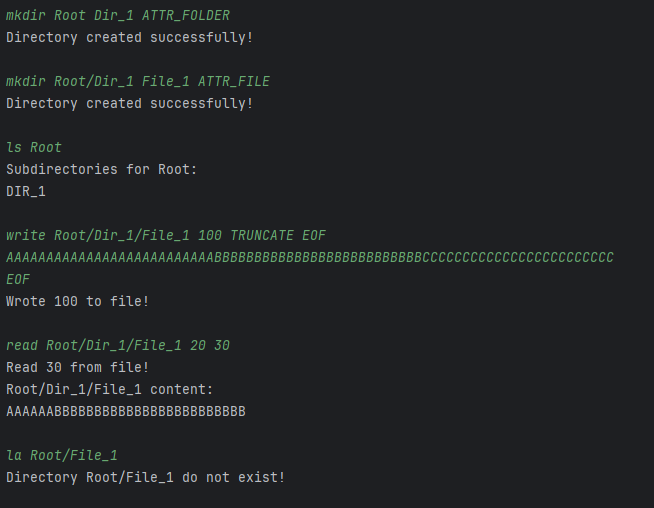
\includegraphics[width=1.0\linewidth]{images/2.5.1.png}
    \label{fig:enter-label}
\end{figure}

\clearpage
\begin{figure}[t!]

    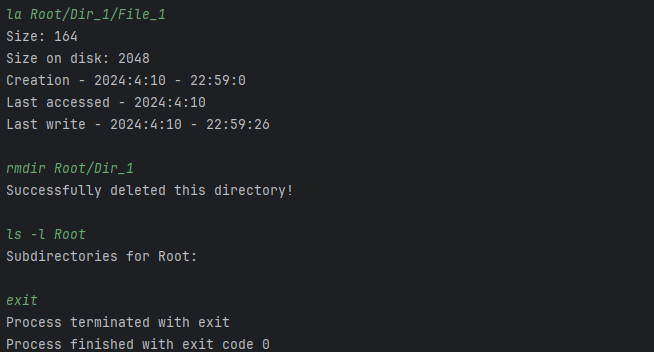
\includegraphics[width=1.0\linewidth]{images/2.5.2.png}
    \label{fig:enter-label}
    \caption{Interacțiunea cu sistemul de fișiere FAT32}
\end{figure}

\bigskip


\subsection{Concluzii FAT32}

În încheiere, FAT32 este un sistem de fișiere relativ simplu, care de-a lungul timpului a dat dovadă de versatilitate și stabilitate, acesta fiind o alegere ideală pentru dispozitivele de stocare de dimensiuni medii. Cu toate acestea, din cauza limitărilor sale, cum ar fi dimensiunea maximă a fișierelor, precum și a securității slabe oferite de acesta, FAT32 poate fi neadecvat pentru stocarea unor fișiere de dimensiuni mari, sau pentru gestionarea datelor sensibile. În concluzie, FAT32 este o alegere ideală datorită compatibilității pe care o ofeăr, însă poate fi limitat de anumite caracteristici ale sale.




















\newpage

\section{Ext2}

\subsection{Privire de ansamblu asupra Ext2}

Ext2 este un sistem de fișiere mai complex decât cel prezentat anterior, acesta împărțind datele într-o serie de grupuri aflate consecutiv în memorie, fiecare astfel de grup, la rândul său, fiind divizat în mai multe regiuni. Aceste grupuri sunt precedate de zona de bootare, care are același rol ca și în cazul FAT32, și anume inițializarea sistemelor calculatorului. O altă componentă esențială a Ext2 o reprezintă inode-urile, fiecare director fiind reprezentat de o astfel de structură.

\begin{itemize}
  \item \textbf{Super block}, această zonă conține o serie de informații legate de sistemul de fișiere, cum ar fi numărul de blocuri dintr-un grup, dimensiunea unui astfel de bloc, sau semnătura specifică Ext2 (0xEF53), aceasta marcând existența sistemului de fișiere în cauză. Deși fiecare grup conține o astfel de zonă, în realitate doar super block-ul primului grup este folosit, celelalte servind drept backup, în cazul în care o corupere de date are loc.

  \item \textbf{Group Descriptors}, regiune de dimensiune variată, care conține, pentru fiecare grup din cadrul sistemului de fișiere, o structură cu informații legate de acesta, cum ar fi numărul de blocuri libere din cadrul său. La fel ca și în cazul superblock-ului, doar zona primului grup este folosită, cele aflate în cadrul celorlalte grupuri reprezintă niște copii redundante, având rol de backup.

  \item \textbf{Block Bit Map}, fiecare bit din cadrul acestui bloc marchează stadiul de ocupare al blocului de date cu indexul corespunzător (0 dacă blocul este liber, sau 1 în caz contrar).

  \item \textbf{Inode Bit Map}, la fel ca și zona anterioară, marchează stadiul de ocupare al inode-urilor din cadrul grupului.

  \item \textbf{Inode Table}, neavând o dimensiune fixă, această zonă conține, pentru fiecare inode prezent în grup, o structură de date cu informații referitoare la acesta, cum ar fi spațiul ocupat, numărul și lista de blocuri, sau tipul directorului pe care îl reprezintă (în cazul implementării noastre există doar 2 tipuri de directoare: folder și fișier simplu).

  \item \textbf{Data Blocks}, în această regiune sunt stocate informațiile propriu-zise din cadrul directoarelor, fiind cea mai amplă zonă din cadrul fiecărui grup.
  
\end{itemize}

\clearpage
\begin{figure}[h!]
    \centering
    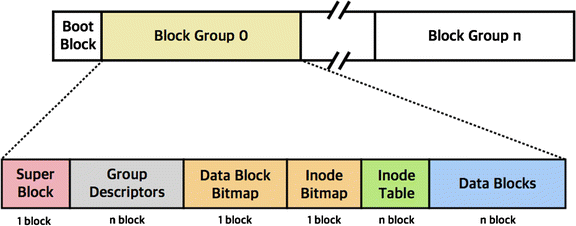
\includegraphics[width=1.0\linewidth]{images/2.6.png}
    \caption{Structura Ext2}
    \label{fig:enter-label}
\end{figure}

\bigskip


\subsection{Modul de implementare}

Similar cu implementarea FAT32, și în cazul Ext2 este vorba despre o simulare, fără ca aceasta să aibă vreo interacțiune directă cu kernel-ul, cum ar face-o un sistem de fișiere adevărat, aflat în cadrul unui sistem de operare. Interacțiunea cu sistemul de fișiere se realizează tot prin intermediul terminalului, comenzile fiind identice cu cele din cadrul FAT32, pentru a avea o oarecare consistență între cele 3 implementări din cadrul acestei lucrări.

\subsubsection{Inițializarea Ext2}

O parte dintre pașii inițializării Ext2 sunt identici cu cei din cadrul FAT32, de aceea aceștia vor fi doar menționați, informații suplimentare fiind oferite doar unde apar diferențe.

\begin{enumerate}
  \item \textbf{Verificarea existenței disk-ului}

  \item \textbf{Inițializarea/Citirea disk-ului}

  \item \textbf{Verificarea inițializării sistemului de fișiere}, ceea ce diferă față de FAT32 este doar semnătura, aceasta fiind 0xEF53.

  \item \textbf{Inițializarea super block-urilor}, etapă ce are loc doar în cazul în care sistemul nu a fost inițializat într-o dată anterioară. Aici, pe baza datelor din cadrul structurii DiskInfo oferite de simularea disk-ului, calculăm valorile anumitor componente din cadrul sistemului, cum ar fi numărul total de inode-uri, numărul total de blocuri sau numărul de blocuri din cadrul unui grup, dar și alte informații precum momentul ultimei scrieri sau numărul de blocuri care trebuie să fie prealocate în momentul creării unui director. De reținut faptul că în cazul ultimului grup aceste valori pot să difere, cel mai probabil având dimensiuni mai reduse decât celelalte grupuri. În final, acest bloc este scris în memorie, pentru fiecare grup în parte.

 \item \textbf{Citirea structurilor de date necesare}, indiferent de rezultatul de la pasul anterior, citim structura de date ext2-super-block, care ne va fi de folos pe parcursul implementării.
 \item \textbf{Inițializarea grupurilor}, etapă ce are loc doar în momentul creării sistemului de fișiere, aici sunt reținute date referitoare la fiecare grup în parte într-o structură ext2-group-desc. Aceste structuri sunt apoi salvate în cadrul regiunii Group Descriptors din cadrul grupurilor.

\item \textbf{Inițializarea directorului rădăcină}, pas ce vine la pachet cu cel anterior, aici prealocăm blocuri directorului rădăcină, cream inode-ul corespunzător, iar mai apoi salvăm în memorie aceste date (vom vorbi mai târziu în detaliu despre modul în care se creează un director).
  
\end{enumerate}

\bigskip

\lstset{style=code-snyppet-style}
\begin{lstlisting}
void ext2Startup(char* diskDirectory, DiskInfo** diskInfo, 
                 uint32_t sectorsNumber, uint32_t sectorSize)
{
    if(checkDiskInitialization(diskDirectory) == false)
        initializeDisk(diskDirectory, diskInfo, sectorsNumber, sectorSize);
    else
        *diskInfo = getDisk(diskDirectory);

    bool ext2AlreadyInitialized = true;
    if(checkExt2FileSystemInitialization(*diskInfo) == false)
    {
        initializeFirstSuperBlockInFirstGroup(*diskInfo);
        ext2AlreadyInitialized = false;
        std::cout << "First super block initialized\n";
    }

    ext2_super_block* firstSuperBlock = readFirstSuperBlock(*diskInfo);

    if(ext2AlreadyInitialized == false)
    {
        initializeGroups(*diskInfo, firstSuperBlock);
        initializeRootDirectory(*diskInfo, firstSuperBlock);
        std::cout << "Groups initialized\n";
    }
}
\end{lstlisting}

\bigskip

\subsubsection{Structura unui director}

Așa cum am menționat și mai devreme, și la fel ca și în cazul FAT32, implementarea noastră are două tipuri de directoare: folder și fișier. Fiecare astfel de director este reprezentat prin intermediul a două structuri de date, ext2-inode, care se află în tabelul de inode-uri din cadrul grupului corespunzător, și ext2-dir-entry, care se află în blocurile de date ale folder-ului părinte. În implementarea originală Ext2, această structură de date are dimensiune dinamică, în funcție de lungimea numelui directorului, însă pentru ușurarea implementării, am decis standardizarea acesteia la 128 bytes, ceea ce presupune un nume de maxim 120 de caractere.

\bigskip

\lstset{style=code-snyppet-style}
\begin{lstlisting}
typedef struct
{
    uint32_t inode;
    uint16_t rec_len;
    uint8_t name_len;
    uint8_t file_type;
    char name[120]; 
} __attribute__((packed)) ext2_dir_entry;
\end{lstlisting}

\bigskip

\subsubsection{Structura blocurile de date din cadrul unui director}

Modul în care blocurile sunt alocate unui director este destul de complex, fiind folosită o împărțire ierarhică a blocurilor pe mai multe nivele. În cadrul inode-ului corespunzător unui director, se află un vector (ce are de obicei lungimea 15) care este împărțit în 4 părți, corespunzătoare celor 4 nivele.

\begin{enumerate}
  \item \textbf{Blocuri directe}, reprezentate de primele 12 valori din cadrul vectorului, fiecare reprezentând index-ul unui bloc.

  \item \textbf{Blocuri indirecte din ordin 2}, elementul din vector aflat pe poziția 12 indică index-ul unui bloc indirect. Acest bloc reprezintă un vector care conține indicii următoarelor blocuri din cadrul directorului. Astfel, acest al doilea nivel conține blocurile din intervalul 12 - (b/4 + 11), unde b reprezintă dimensiunea unui bloc în bytes.

  \item \textbf{Blocuri indirecte din ordin 3}, elementul din vector aflat pe poziția 13 indică spre un tabel de ordin 2, elementele acestuia indicând spre o listă de tabele de ordin 3, acestea conținând indicii următoarelor blocuri, aflate în intervalul b/4 + 12 -  (b/4)*(b/4) + b/4 + 11.

  \item \textbf{Blocuri indirecte din ordin 4}, elementul din vector aflat pe poziția 14 indică spre un tabel de ordin 2, care indică spre o listă de tabele de ordin 3, acestea din urmă indicând spre o listă de tabele de ordin 4, ce conțin indicii ultimelor blocuri din cadrul directorului, aflate în intervalul (b/4)*(b/4) + b/4 + 12 - (b/4)*(b/4)*(b/4) + (b/4)*(b/4) + b/4 + 12.

\end{enumerate}

\begin{figure}[h!]
    \centering
    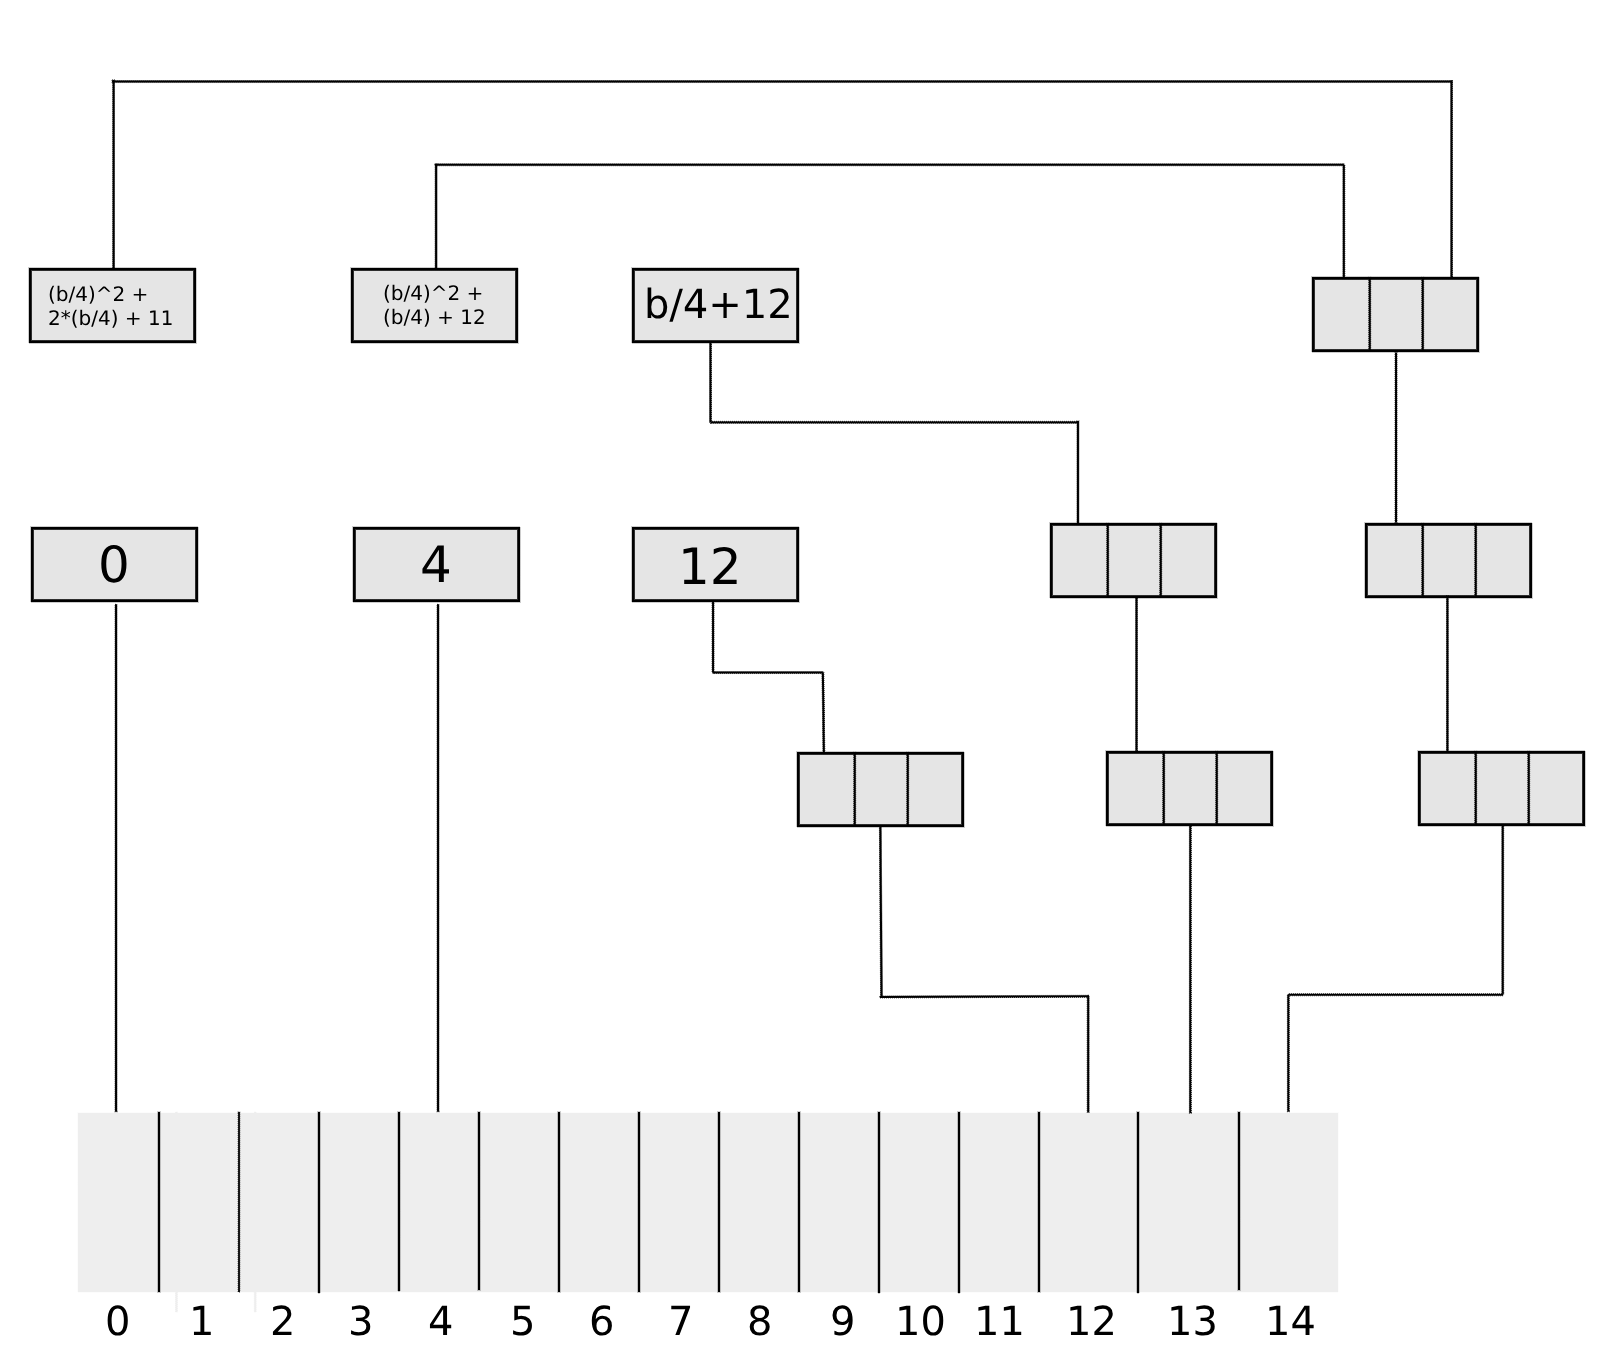
\includegraphics[width=0.9\linewidth]{images/2.7.png}
    \caption{Împărțirea blocurilor pe nivele}
    \label{fig:enter-label}
\end{figure}

\bigskip


\subsubsection{Crearea unui director}

Pentru crearea unui director, sunt folosiți o serie de algoritmi pentru a decide unde să fie alocat inode-ul corespunzător acestuia, și totodată blocurile de date inițiale:

\begin{enumerate}
  \item \textbf{Directorul este de tip folder}, în acest caz, algoritmul de căutare al inode-ului implementează două euristici:
  
  \begin{enumerate}
      \item Folderele care au ca și director părinte directorul rădăcină trebuie să fie împrăștiate în toate grupurile. Astfel, funcția noastră caută un grup având numărul de inode-uri libere și numărul blocurilor libere peste medie. Dacă niciun astfel de grup nu este găsit, se sare la pasul c.

      \item Folderele care nu au ca și director părinte directorul rădăcină trebuie puse în grupul în care se află părintele acestora, dacă satisface următoarea regulă: se folosește o valoare 'debt' care reprezintă diferența dintre numărul de foldere și numărul de fișiere din cadrul directorului, iar această valoare este mai mică decât media 'debt-ului' celorlalte grupuri.

      \item Regula de 'fallback', utilizată în cazul în care condițiile pentru celelalte 2 nu sunt îndeplinite. Funcția caută un grup în care numărul inode-urilor disponibile este mai mare decât media.
  \end{enumerate}

  \item \textbf{Directorul este de tip fișier}, in acest caz, sunt implementate 2 euristici:

  \begin{enumerate}
      \item Se realizează o căutare logaritmică începând cu grupul care conține inode-ul directorului părinte. Algoritmul caută log(n) blocuri, unde n reprezintă numărul total de grupuri. Astfel, sunt verificate grupurile: i mod (n), (i + 1) mod (n), (i + 1 + 2) mod (n), (i + 1 + 2 + 4) mod (n) (unde i reprezintă index-ul blocului părinte), până când este găsit un grup ce conține inode-uri libere.
      
      \item Dacă nu este găsit niciun grup care să conțină inode-uri libere folosind euristica de mai sus, se caută un grup disponibil în mod liniar, începând cu primul.
  \end{enumerate}

\end{enumerate}

\bigskip

\lstset{style=code-snyppet-style}
\begin{lstlisting}
if(fileType == FILE_TYPE_FOLDER)
   searchInodeResult = (isParentRoot ? searchFreeInodeForDirectoryHavingParentRoot(diskInfo, superBlock,                                                   inodeGlobalIndex) :
   searchFreeInodeForNestedDirectory(diskInfo, superBlock, parentInode,                             
                                     inodeGlobalIndex));
else if(fileType == FILE_TYPE_REGULAR_FILE)
   searchInodeResult = searchFreeInodeForRegularFile(diskInfo, superBlock, parentInode, inodeGlobalIndex);
\end{lstlisting}

\bigskip

După găsirea și scrierea în memorie a inode-ului, trebuie găsite și prealocate o listă de blocuri pentru noul director. Astfel, fiind dat un număr de blocuri care să fie prealocate (în cazul implementării noastre această valoare este 8), sunt urmați următorii pași:

  \begin{enumerate}
      \item Se încearcă găsirea a n (inițial n = 8) blocuri libere consecutive. Prima dată aceste blocuri sunt căutate în grupul în care a fost alocat inode-ul, iar dacă acest lucru nu este posibil, se sare la pasul 2.
      
      \item Sunt parcurse în mod liniar toate blocurile, începând cu primul, până când sunt găsite 8 blocuri consecutive. Dacă nici asta nu reușește, se trece la pasul următor.

      \item Numărul de blocuri care trebuie prealocate este înjumătățit (pentru n inițial = 8 -> 4 -> 2 -> 1), și se reia pasul 1.
  \end{enumerate}

După ce au fost realizați acești pași, în final se adaugă un nou ext2-dir-entry folder-ului părinte, se actualizează datele temporale legate de ultima accesare din cadrul inode-ului acestuia, sunt actualizați descriptorii, atât pentru grupul în care a fost creat noul inode, cât și pentru cel în care au fost prealocate blocurile pentru acesta, același lucru întâmplat și în cazu; bit map-urile corespunzătoare.

\subsubsection{Căutarea unui director}

Căutarea unui director se realizează într-o manieră recursivă. Se pornește din directorul rădăcină, fiind parcurse ext2-dir-entry-urile din cadrul tuturor folderelor aflate în path-ul dat, până când este găsit directorul cu denumirea dorită.

\subsubsection{Scrierea fișierelor}

Ca și în cazul FAT32, există două moduri de scriere a unui fișier, și anume APPEND și TRUNCATE. În cadrul acestei operațiuni, sunt utilizate mai întâi blocurile prealocate, urmând ca unele noi să fie atribuite fișierului, în cazul în care numărul de bytes care se dorește a fi scris este mai mare decât capacitatea actuală a directorului.

Un lucru important de menționat aici este faptul că în momentul în care se realizează o scriere în modul TRUNCATE, iar dimensiunea fluxului de date este mai mică decât mărimea actuală a fișierului, blocurile devenite neocupate nu sunt dealocate! Spre exemplu, dacă avem un fișier de dimensiune 10.000 (bytes), acesta conține 10 blocuri; efectuăm o operațiune de scriere a 6000 de bytes în modul TRUNCATE, ceea ce presupune utilizarea a numai 6 blocuri, astfel 4 urmând să devină neocupate, rămânând în continuare alocate fișierului în cauză. Această decizie a fost luată pentru a putea observa mai bine diferențele dintre timpul necesar scrierii unui fișier în care toate blocurile necesare sunt deja prealocate, față de o scriere care presupune și alocarea unor blocuri de date suplimentare.

\subsubsection{Citirea fișierelor}

Citirea datelor dintr-un fișier se realizează prin parcurgerea blocurilor din cadrul acestuia, până când numărul de bytes dorit este acoperit. La fel ca și în cazul sistemului de fișiere precedent, citirea poate fi realizată atât în totalitate, cât și parțial, utilizatorului fiindu-i oferită posibilitatea de a preciza un index de start care să reprezinte poziția de început a citirii.

\subsubsection{Dealocarea blocurilor de date}

Așa cum am precizat mai sus, în cazul unei scrieri în modul truncate, blocurile rămase neocupate nu sunt dealocate. Dacă totuși dorim să reducem dimensiunea unui fișier, și totodată să eliberăm o parte din blocurile alocate acestuia, avem la dispoziție operația de truncate.

\subsubsection{Ştergerea directoarelor}

Ștergerea directoarelor poate reprezenta un proces destul de complex, mai ales în cazul folderelor, deoarece această operațiune nu presupune doar ștergerea directorului în cauză, ci și a tuturor descendenților direcți, cât și indirecți ai săi. Pe scurt, acest lucru presupune dealocarea blocurilor de date, marcarea acestora ca libere în cadrul bitmap-urilor pentru blocuri, ștergerea inode-urilor și marcarea acestora ca disponibile, actualizarea descriptorilor grupurilor aferente, cât și ștergerea ext2-dir-entry-ului din cadrul folder-ului părinte.

\subsection{Interacțiunea cu utilizatorul}

Interacțiunea cu sistemul de fișiere se realizează în mod similar ca în cazul FAT32, comenzile fiind identice. Pentru Ext2 există totuși o comandă în plus, care are rolul de a prealoca în avans blocuri pentru un fișier dat:

\bigskip

\textbf{preallocate (Nume fișier) (Număr bytes)} \textit{preallocate Root/MyFile 8000} - adaugă fișierului în cauză suficiente blocuri cât să încapă numărul de bytes specificat. În exemplul dat, dacă dimensiunea unui bloc este de 1024 bytes, fișierului în cauză îi vor fi adăugate 8 blocuri.

\bigskip

\begin{figure}[h]
    \centering
    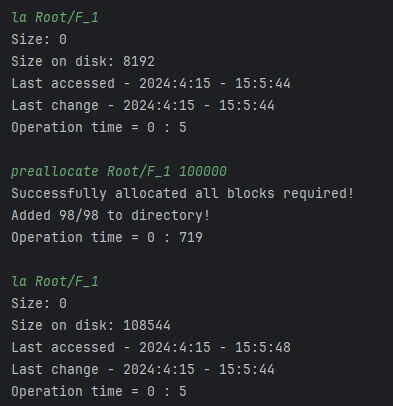
\includegraphics[width=0.7\linewidth]{images/2.8.png}
    \caption{Utilizarea comenzii \textit{preallocate}}
    \label{fig:enter-label}
\end{figure}

\subsection{Concluzii Ext2}

În concluzie, Ext2 este un sistem de fișiere robust, oferind un mod eficient de stocare și gestionare a datelor în cadrul unui sistem de calcul, acesta fiind cunoscut în special pentru utilizarea sa în cadrul sistemului de operare Linux. Cu toate că a fost înlocuit în mare măsură de versiunile mai noi precum Ext3 și Ext4, Ext2 rămâne în continuare un sistem de fișiere larg utilizat, datorită simplității sale și stabilității de care a dat dovadă de-a lungul timpului.